\subsection{Continuum Procedure}\label{sec:continuum}

\todo{Make this just about the contact operator, not a tower.}

The starting point are interactions given by a tower of derivative contact operators such that the tree amplitude in the center of mass frame is given by
\begin{equation}
    V(p) = + i\sum_n C_{2n}(\Lambda) p^{2n}
\end{equation}
where $p$ denotes the relative momentum of incoming nucleons and the interaction strengths $ C_{2n}(\Lambda)$ depend on the regulator $\Lambda$ and carry dimension-dependent units.
The scattering amplitude is given by the bubble sum depicted in \Figref{bubbleSum}.

\begin{figure}[ht!]
\center
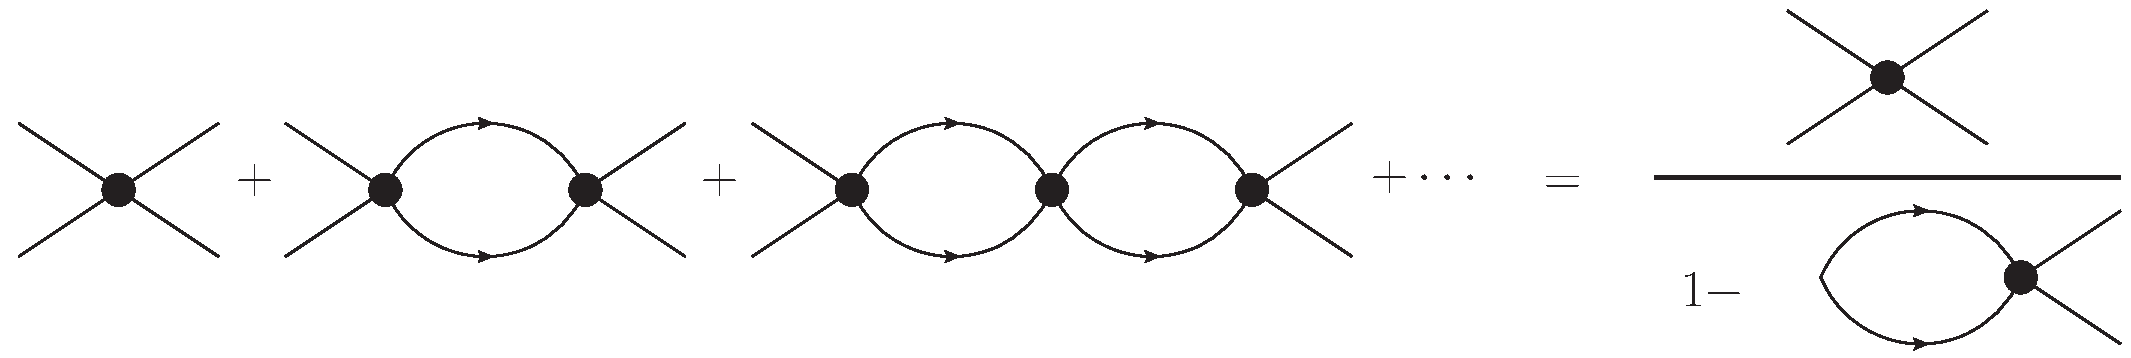
\includegraphics[width=\columnwidth]{figure/bubbleSum.pdf}
\caption{Bubble sum. Each line represents a propagator, each vertex represents $-i \sum_n C_{2n}(\Lambda) p^{2n}$, and the bubble is given by $I_0$ (see also \Figref{I0}).\label{fig:bubbleSum}}
\end{figure}

This bubble sum is a geometric series and, restricting our attention to the s-wave, gives, for the standard $T$-matrix, \cite{Kaplan:1998we,Beane:2003da}
\begin{equation}\label{eq:T matrix}
iT(p) = \frac{-i\sum_n C_{2n}(\Lambda) p^{2n}}{1-I_0(p,\Lambda) \sum_n C_{2n}(\Lambda) p^{2n}},
\end{equation}
where $p$ is the relative momentum, $\Lambda$ the dimensional regularization scale,  and $I_0(p,\Lambda)$ is a $D$-dependent function that arises from integrating the loop shown in \Figref{I0},
\begin{align}
    I_0(p)
    &=-i\int^{\Lambda}
        \frac { \mathrm {d}q_0}{2\pi}\ \frac{\mathrm { d } ^ { D } \vec{ q } } { (2\pi)^ { D } }
        \left( \frac { i } { \frac{E}{2} + q _ { 0 } - \frac{\vec{q}^2}{2m_1} + i \epsilon } \right)
        \left( \frac { i } { \frac{E}{2} - q _ { 0 } - \frac{\vec{q}^2}{2m_2} + i \epsilon } \right)
    \label{eq:I0 in two particle language}\\
    &=\frac{\Omega_D}{(2\pi)^D}\int^{\Lambda}  \mathrm { d } q \ q^{D-1}\left[\PV \left( \frac { 1 } { E - \frac{\vec{q}^2}{2\mu} } \right)
-i\frac{\pi \mu}{q}\delta(q-\sqrt{2 \mu E})\right]
    \label{eq:I0 in relative coordinates}
    \\
    &=\frac{\Omega_D}{(2\pi)^2}\frac{2\mu}{L^{D-2}}\int^{\Lambda L/2\pi}  \mathrm { d } n \ n^{D-1}\left[\PV \left( \frac { 1 } { \left(\frac{pL}{2\pi}\right)^2 - n^2 } \right)
-i\frac{\pi^2}{L n}\delta\left(\frac{2\pi}{L}n -p\right)\right]
    \label{eq:I0}
\end{align}
where $\PV$ refers to Principal (Cauchy) Value, we have used the on-shell condition $2\mu E=p^2$, and the geometric factor
\begin{equation}
\Omega_D=\frac{2\pi^{D/2}}{\Gamma(D/2)}=
    \begin{cases}
        4\pi    &   (D=3)\\
        2\pi    &   (D=2)\\
        2       &   (D=1)
    \end{cases}\ ,
\end{equation}
accounts for the angular integration in $D$ dimensions.

\begin{figure}[h!]
    \center
    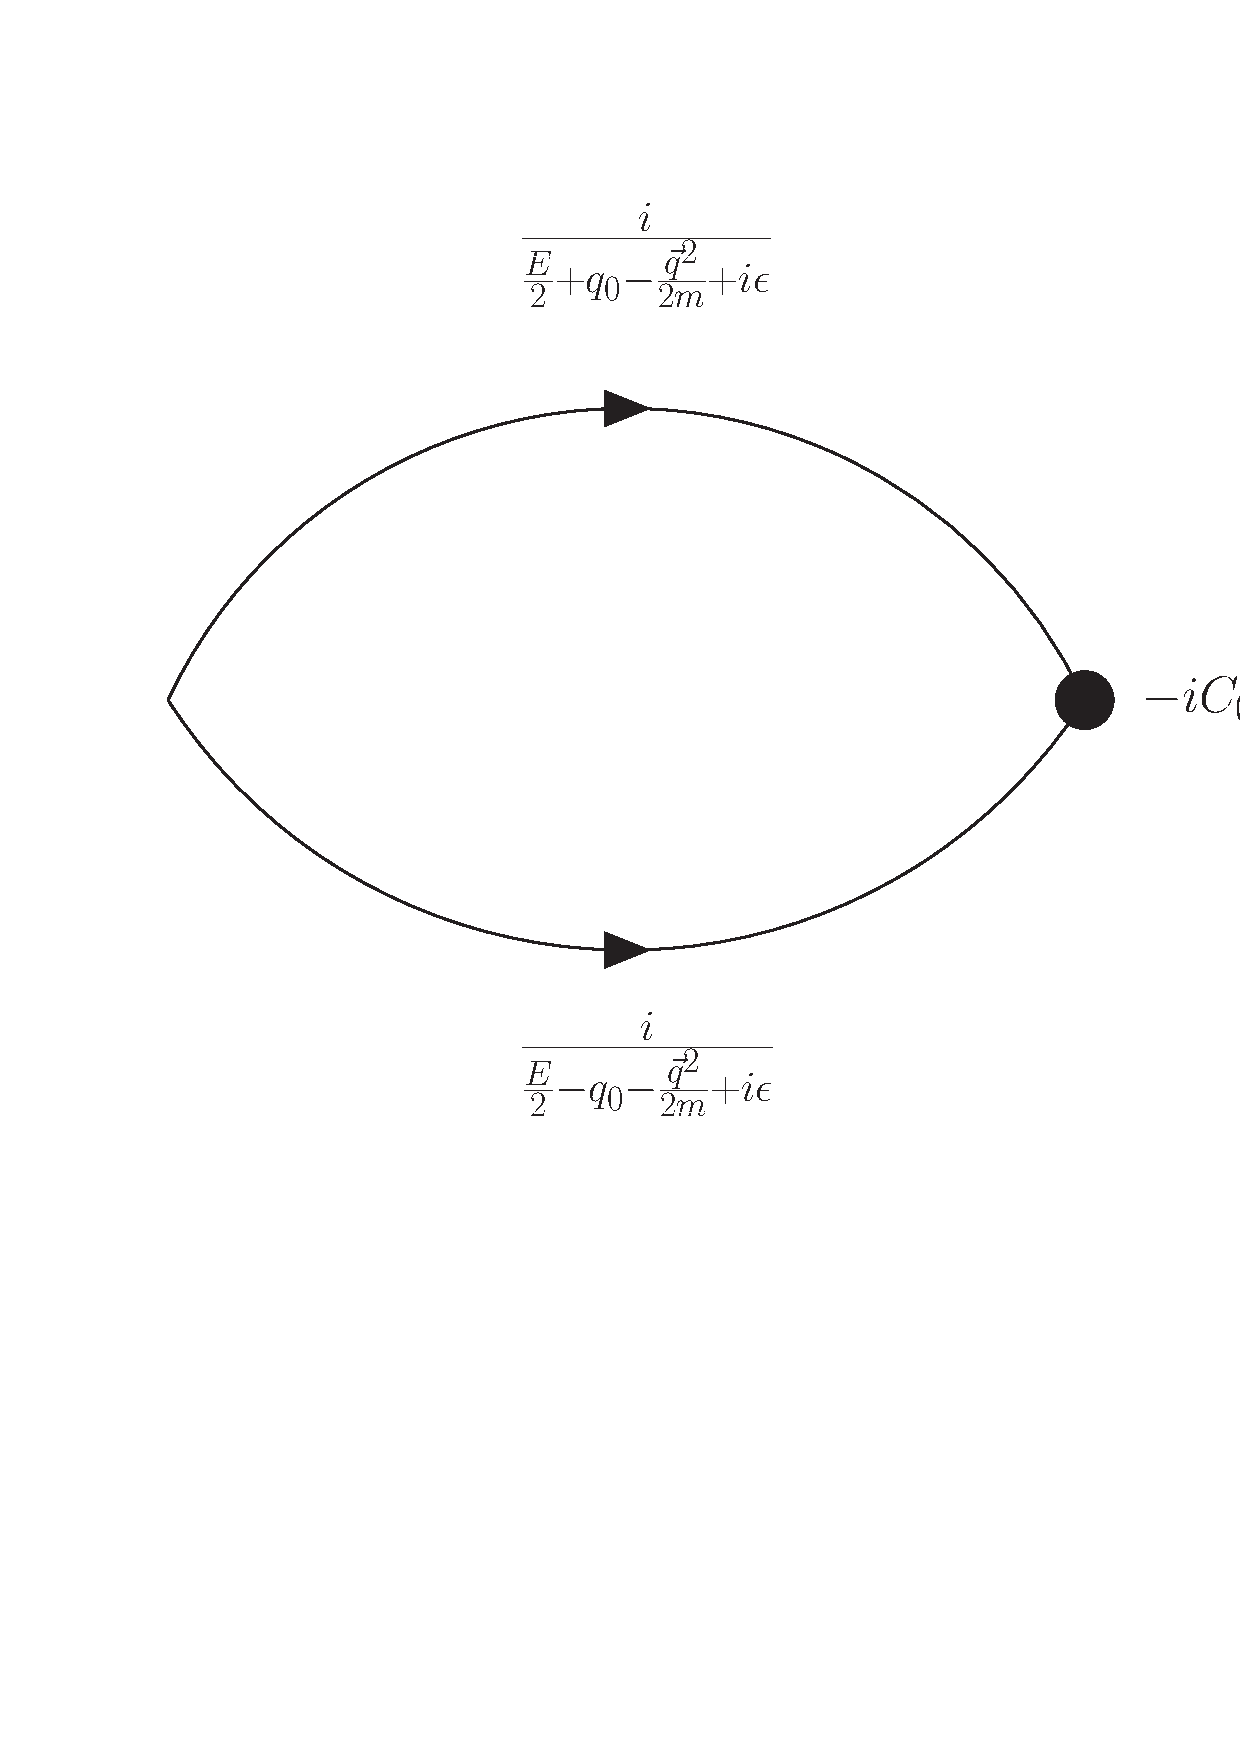
\includegraphics[width=.5\columnwidth]{figure/I0.pdf}
    \caption{
        Loop diagram contributing to the bubble sum.
    }
    \label{fig:I0}
\end{figure}

In the $s$-wave, the momentum-dependent $T$-matrix is related to the phase shift $\delta_0(p)$ by
\begin{equation}\label{eq:cot delta}
    i T = \frac{2}{\mu}\F_{D}\frac{i}{\cot \delta_0(p)-i}\ ,
\end{equation}
where
\begin{equation}\label{eq:spherical FD}
    \F_{D} \equiv \F_{0D}
    =
    \begin{cases}
        \pi/p   & (D=3)\\
        1       & (D=2)\\
        p/2     & (D=1)
\end{cases}
\end{equation}
is a dimension-dependent kinematic factor.
This fixes the coefficients $C(\Lambda)$ as a function of the scattering data,
\begin{equation}\label{eq:IV pole}
    \frac{1}{\sum_n C_{2n}(\Lambda) p^{2n}}
    =
    I_0(p) - \frac{\mu}{2 \F_D}\left(\cot \delta_0(p) - i\right)
\end{equation}

In a finite volume, the energy eigenstates $E$ appear at poles of the $T$-matrix, so that
\begin{equation}\label{eq:FV pole}
    \frac{1}{\sum_n C_{2n}(\Lambda) (2\mu E)^{2n}} - I_{0,\FV}(2\mu E,L) = 0
\end{equation}
and the infinite-volume integral $I_0$ has been replaced by the matching finite-volume sum,
\begin{align}
I_{0,\FV}(2\mu E,L)
    &=-i\int \frac { \mathrm {d}q_0}{2\pi} \frac{1}{L^D}\sum_{\vec{q}}^{q < \Lambda} \left( \frac { i } { \frac{E}{2} + q _ { 0 } - \frac{\vec{q}^2}{2m_1} + i \epsilon } \right) \left( \frac { i } { \frac{E}{2} - q _ { 0 } - \frac{\vec{q}^2}{2m_2} + i \epsilon } \right)
    \\
    \label{eq:I0 FV}
    &=\frac{1}{L^D}\sum_{\vec{q}}^{q < \Lambda} \frac { 1 } { E - \frac{\vec{q}^2}{2\mu} }
    =\frac{2\mu}{(2\pi)^2 L^{D-2}} \sum_{\vec{n}}^{n < \frac{\Lambda L}{2\pi}} \frac{1}{x-n^2}
    &
    x &= \frac{2\mu E L^2}{4\pi^2}
    \, .
\end{align}
Combining the infinite-volume and finite-volume relations \eqref{IV pole} and \eqref{FV pole} yields
\begin{equation}\label{eq:spherical zeta}
    \frac{\mu}{2\F_D}(\cot\delta_0(2\mu E)-i) = I_0(2\mu E) - I_{0,\FV}(2\mu E),
\end{equation}
the finite-volume quantization condition.
Note that both equations are explicitly evaluated for the same interactions using the same regulator and furthermore \eqref{spherical zeta} is only valid if evaluated at momenta corresponding to finite-volume eigenenergies $E$.

Plugging our results for the integrals in, one finds
\begin{equation}
    \frac{1}{2\F_D}\left(\cot \delta_0(2\mu E) - i\right) = \frac{2}{(2\pi)^2 L^{D-2}}\left[ \left(\int_{\vec{n}} - \sum_{\vec{n}}\right) \frac{1}{x-n^2} + \frac{-i \pi^2\Omega_D}{L} \int \mathrm{d}n\ n^{D-2} \delta\left(\frac{2\pi}{L}n - 2\mu E\right) \right]
\end{equation}
where both the sum and integral are cut off by a restriction on the magnitude of $n$, $n^2 < (\Lambda L / 2\pi)^2$, and the integral implicitly carries a factor of $\Omega_D n^{D-1}$.
In a seemingly miraculous (but required) cancellation, the imaginary part on the left hand side exactly cancels the last term in the sum on the right,\footnote{Actually, the cancellation is not \emph{so} miraculous---demanding it occur is essentially how $\F_D$ is determined.} and we are left with
\begin{equation}
    \cot \delta_0(p) = \frac{\F_D}{\pi^2 L^{D-2}} \left(\sum_{\vec{n}}-\int_{\vec{n}}\right) \frac{1}{n^2-x}
\end{equation}
with $x$ as in \eqref{I0 FV} and we switched the sign of the sum and integral as well as the sign of the denominator.
Because we cut off the sum and the integral in exactly the same way, in dimensions where $I_0$ diverges with $\Lambda$, the divergence cancels against the divergence in the sum.
Let $N=\Lambda L/\pi$.
Then, defining, with a finite cutoff on magnitude $N/2$,
\begin{equation}\label{eq:spherical cutoff S}
    S^{\spherical N}_D(x) = \left(\sum_{\vec{n}}- \int_{\vec{n}}\right) \frac{1}{n^2-x}
\end{equation}
where the $\spherical$ superscript reminds us that we cut off our sum and integral in a spherical way, based on the magnitude of $n<N/2$, we recover the usual \Luscher zeta functions by taking
\begin{equation}\label{eq:spherical S}
    S^\spherical_D(x)
    =
    \lim_{N\goesto\infty} S^{\spherical N}_D(x)
    =
    \lim_{N\rightarrow\infty}\left( \sum_{\vec{n}}^{n < N/2} \frac{1}{n^2-x} - \counterterm_D^\spherical \left(\frac{N}{2}\right)^{D-2}\right)
\end{equation}
where dimension-dependent counterterm $\counterterm_D^\spherical$ comes from the integral; we evaluate the spherical-cutoff integrals and extract said counterterms in \Appref{counterterm/spherical}.\footnote{
In higher dimensions there will be additional divergences which cancel, for example, in five spatial dimensions there will be a cubic and linear divergence.
}
Finally,
\begin{equation}\label{eq:spherical quantization}
    \cot \delta_0(p) = \frac{\F_D}{\pi^2 L^{D-2}} S^\spherical_D(x)
\end{equation}
where we traded the energy dependence for momentum on the left-hand side.
This is the usual \Luscher finite-volume quantization condition, and continuum energy levels should be fed through it to produce continuum scattering data.
In three dimensions it is common to move the momentum dependence in $\F_D$ to the other side, as $p \cot\delta_0(p)$ is what appears in the effective range expansion, as mentioned in \eqref{ere}.
In two dimensions, it will prove useful to explicitly separate the logarithmic divergence, and we will rearrange this equation and slightly redefine $S^\spherical_2$ as needed in \Secref{2D}.

Derived in the zero-temperature continuum, only cold continuum-extrapolated spectra ought to be fed through \eqref{spherical quantization} to extract continuum phase shifts.

To approach the continuum limit, the authors of \Ref{Lee:2007ae} proposed tuning the interaction until the ground state, when fed through $S^\spherical$, produced the desired amplitude that corresponds to the desired scattering length.
We will show in \Secref{3D} that this procedure induces a momentum dependence in the scattering amplitude sensitive to discretization.
In the next subsection we give a procedure that produces a momentum-independent amplitude as one approaches the continuum, and discuss the limiting procedure itself.
